\chapter{Robot Details}

In this chapter we will examine the robot's architecture and details.

\section{Hardware}

The robot in discussion includes two encoders and an IMU in order to have motion's observation and be able, in the firmware's logic, to compute the odometry of the robot.\\
We have used :
\begin{itemize}
	\item a Mega2560 board\supercite{mega2560_datasheet},
	\item two rotary encoders KY-040\supercite{enc_datasheet},
	\item an IMU 10DOF MPU 9250\supercite{imu_prod_spec}.
\end{itemize}


\begin{figure}[htb]
 \centering
	\begin{subfigure}{0.3\textwidth}
		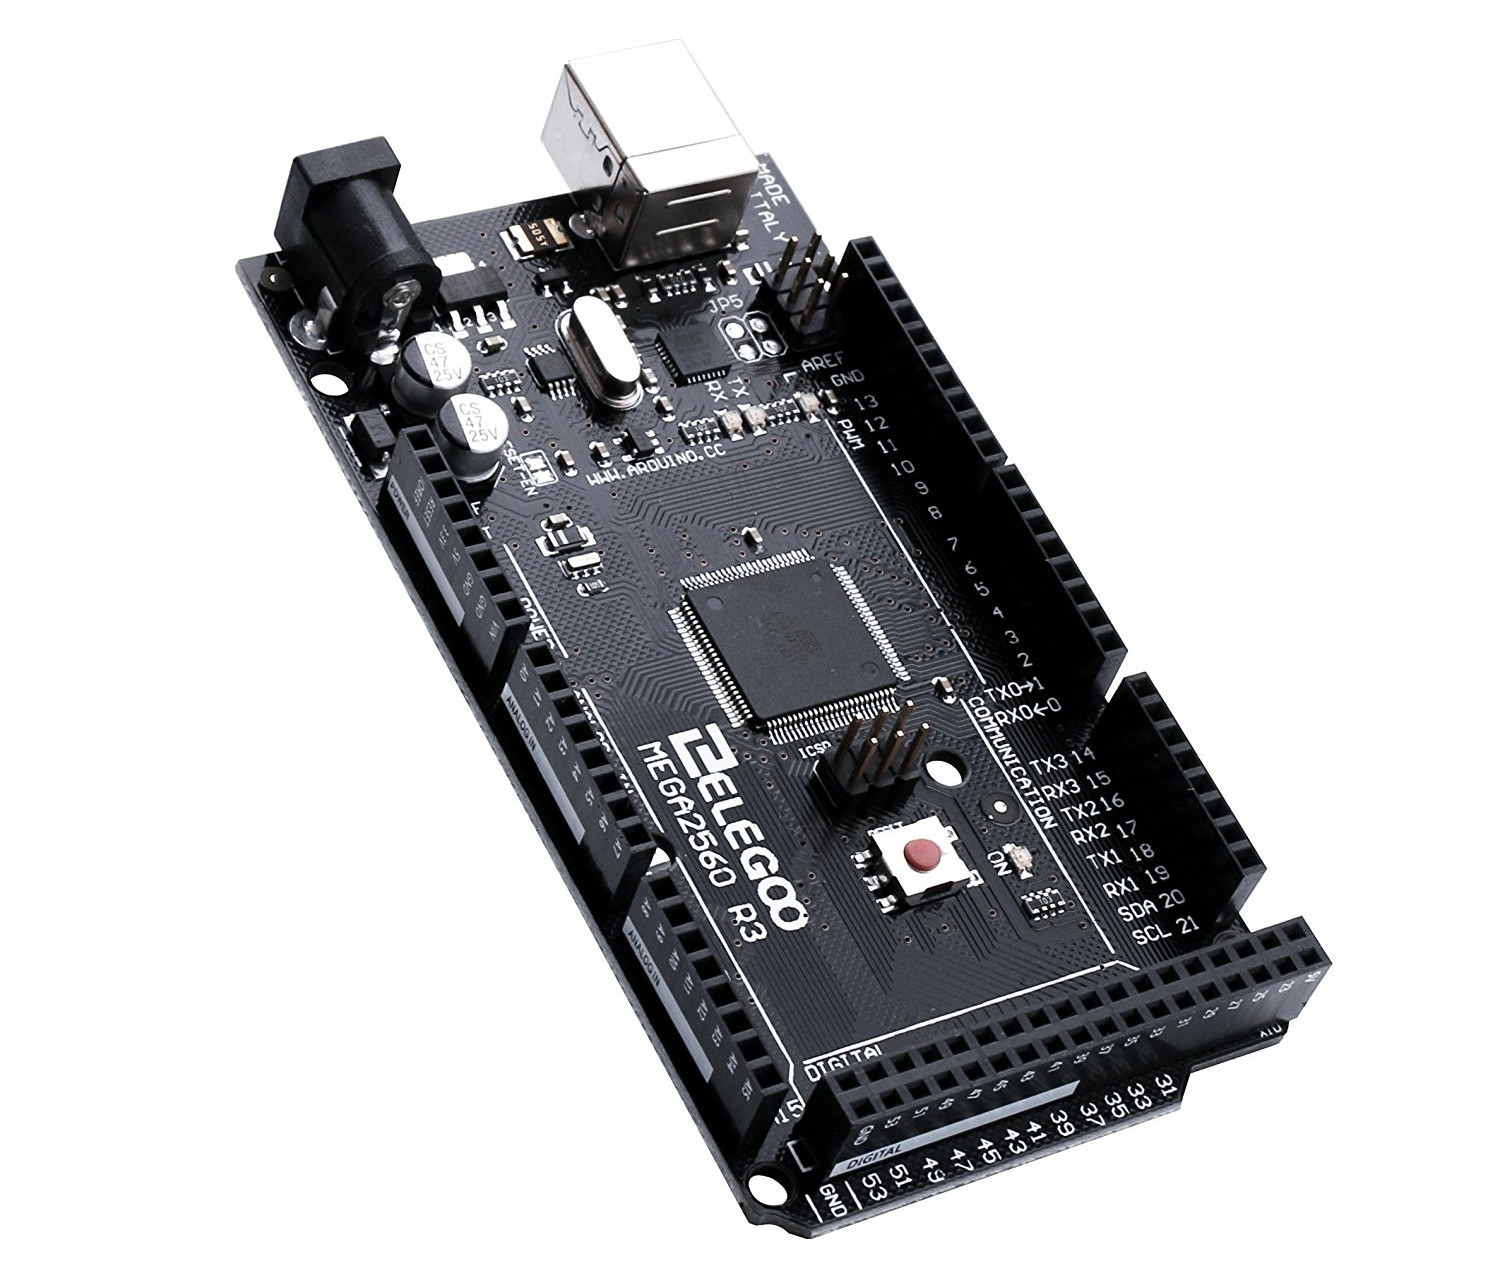
\includegraphics[width=\linewidth]{mega2560_00}
		\captionsetup{justification=centering}
		\caption{A Mega2560 board,}
	\end{subfigure}\hfil
	\begin{subfigure}{0.3\textwidth}
		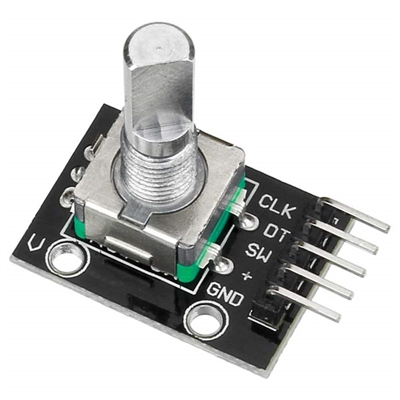
\includegraphics[width=\linewidth]{encs_ky_040}
		\captionsetup{justification=centering}
		\caption{two rotary encoders KY-040,}
	\end{subfigure}\hfil
	\begin{subfigure}{0.3\textwidth}
		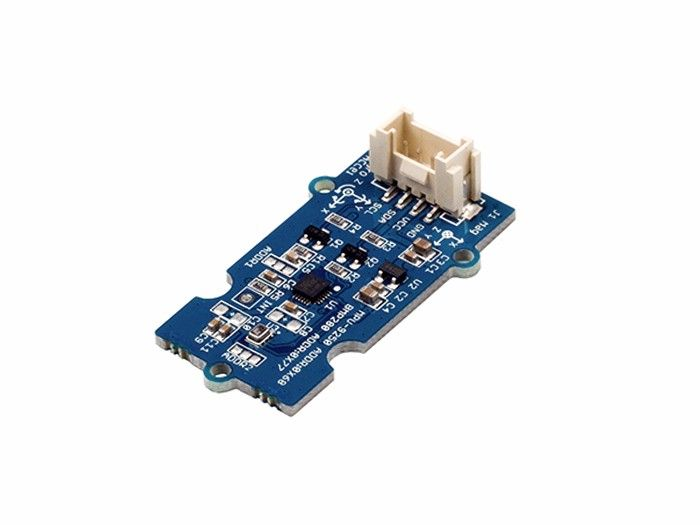
\includegraphics[width=\linewidth]{imu_mpu9250}
		\captionsetup{justification=centering}
		\caption{an IMU 10DOF MPU 9250.}
	\end{subfigure}
	\captionsetup{justification=centering, margin=1.5cm}
	\centering
	\caption{Hardware used for the robot.}
\end{figure}
The encoders are connected to the wheels in order to measure the wheels' rotations, while the IMU is mounted in correspondence of the center of the robot (where as center of the robot we take the mid-point of the wheel axle) at a higher position in order to reduce the electromagnetic-noise given by the CPU computations.\\
\begin{figure}[htb]
 \centering
	\begin{subfigure}{0.43\textwidth}
		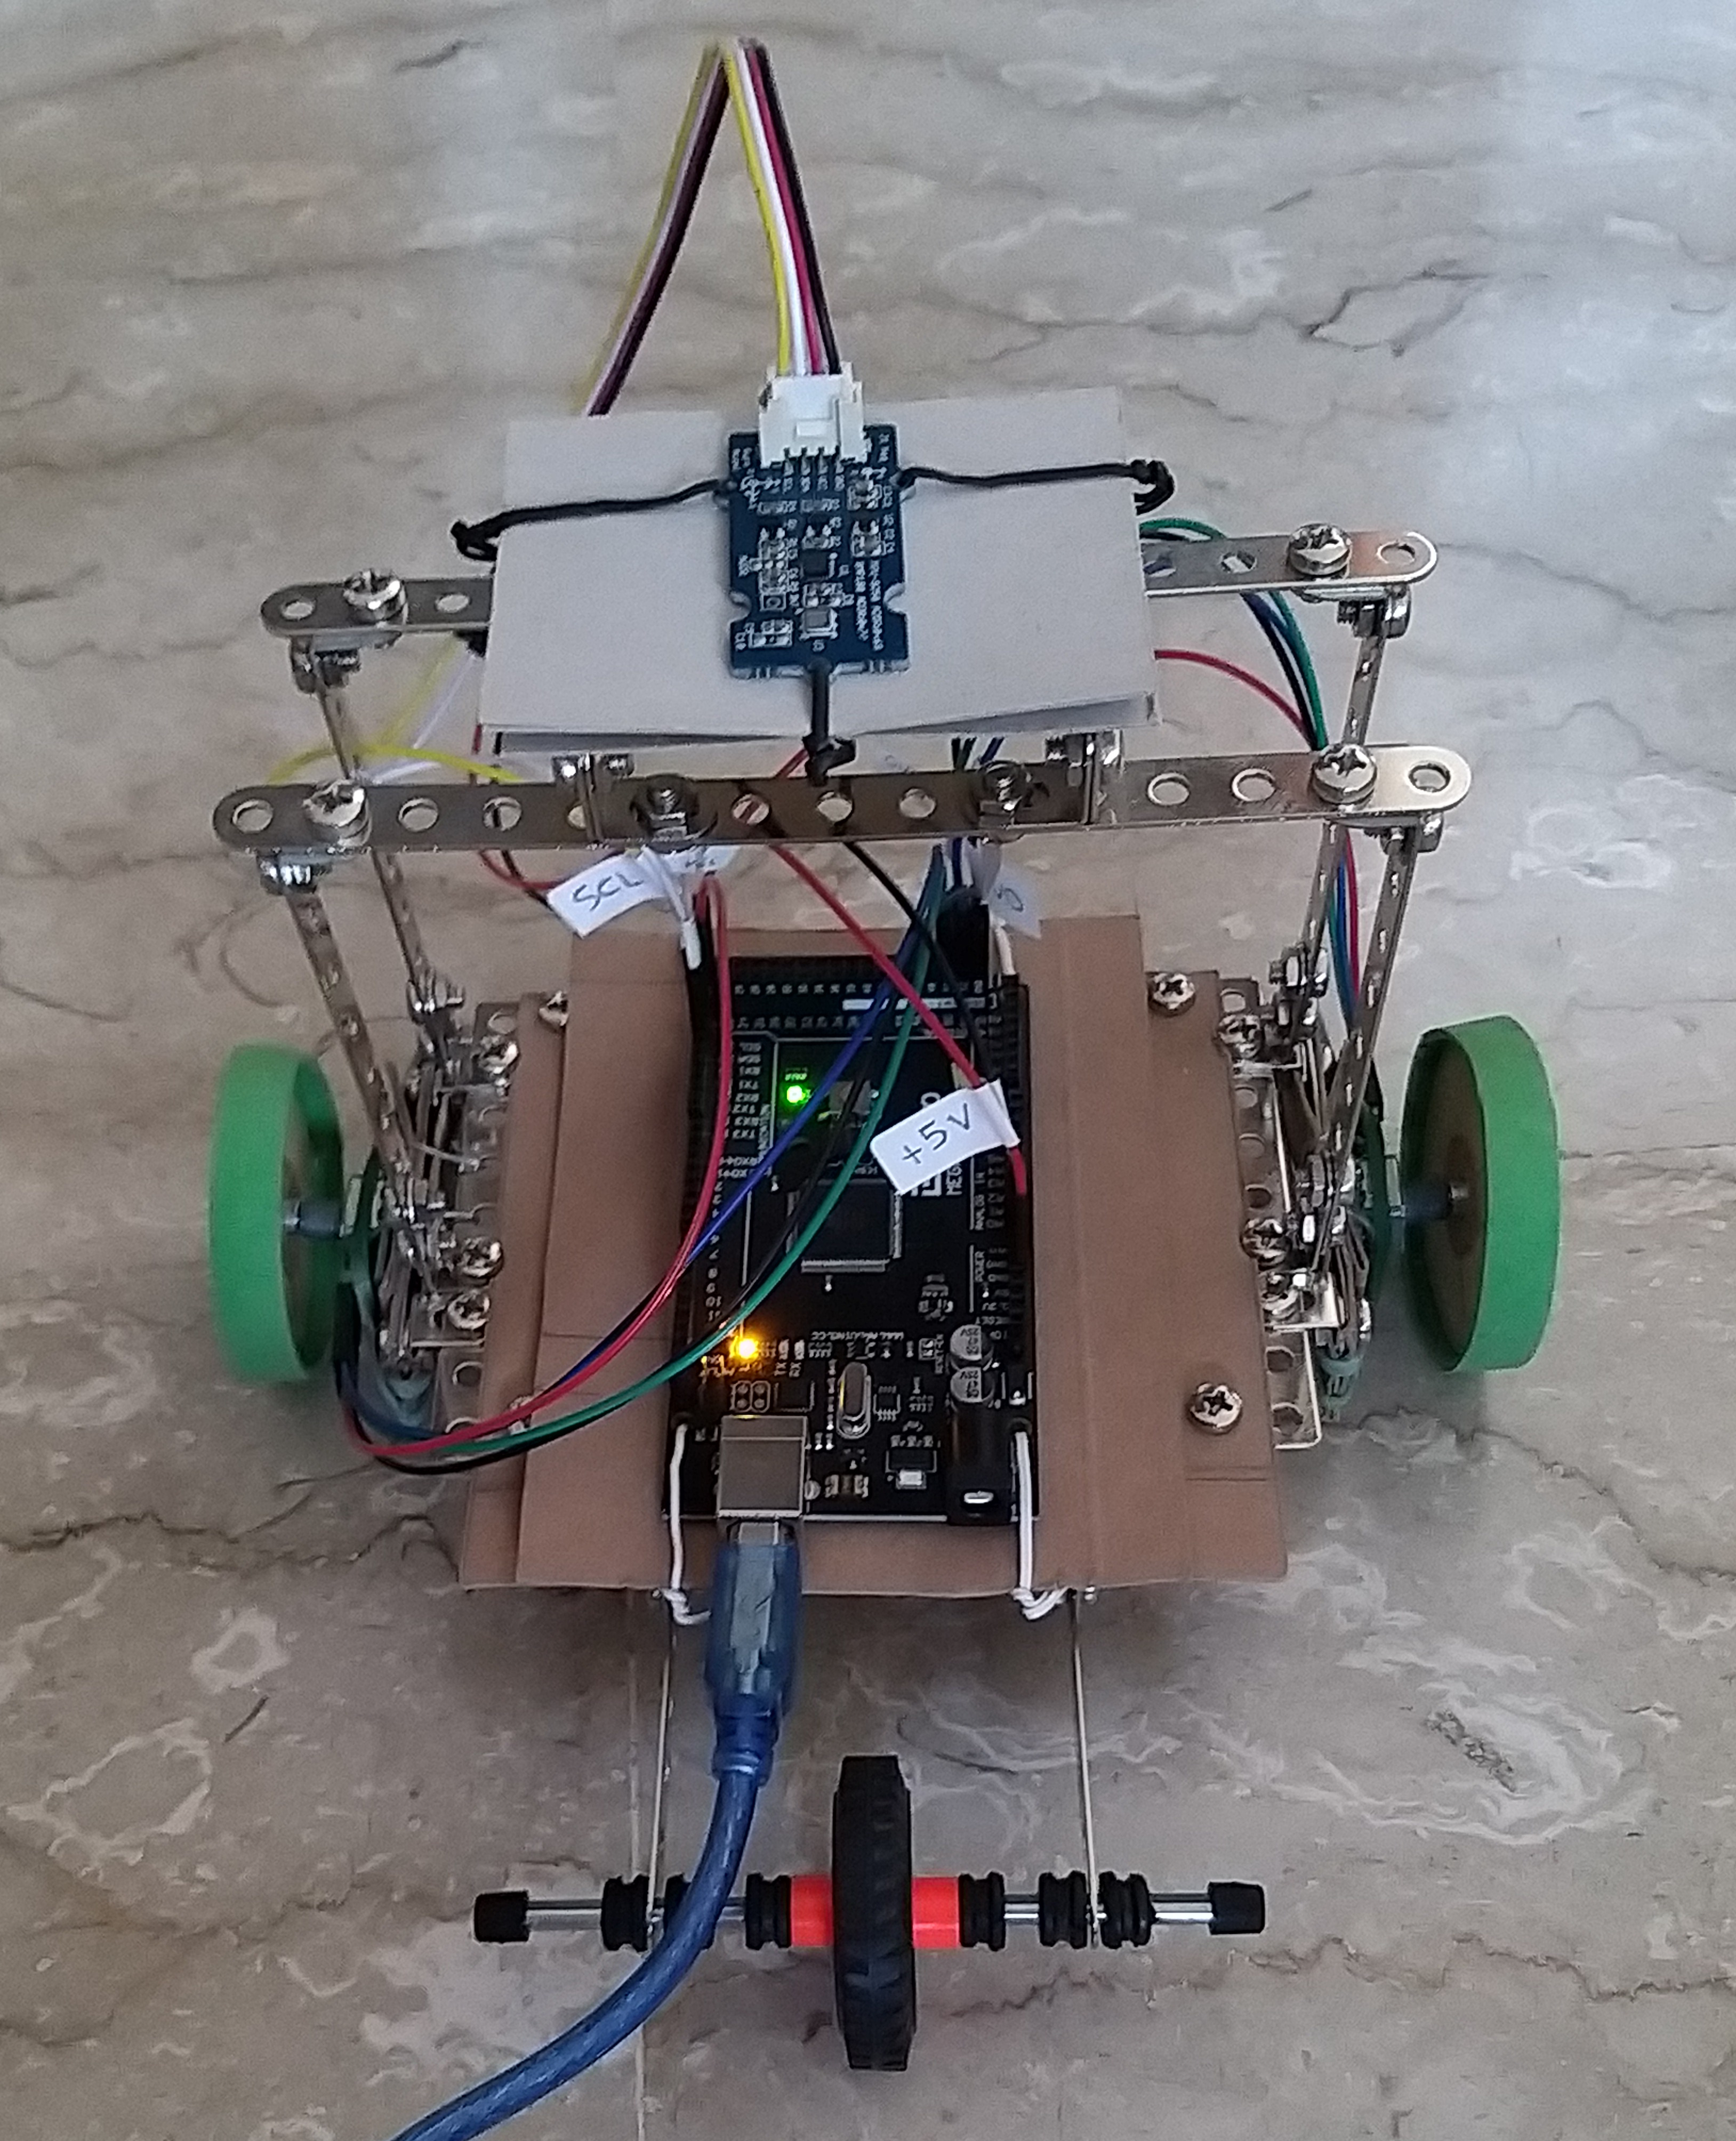
\includegraphics[width=\linewidth]{robot_image_01_20190701_085754_001}
	\end{subfigure}\hfil
	\begin{subfigure}{0.47\textwidth}
		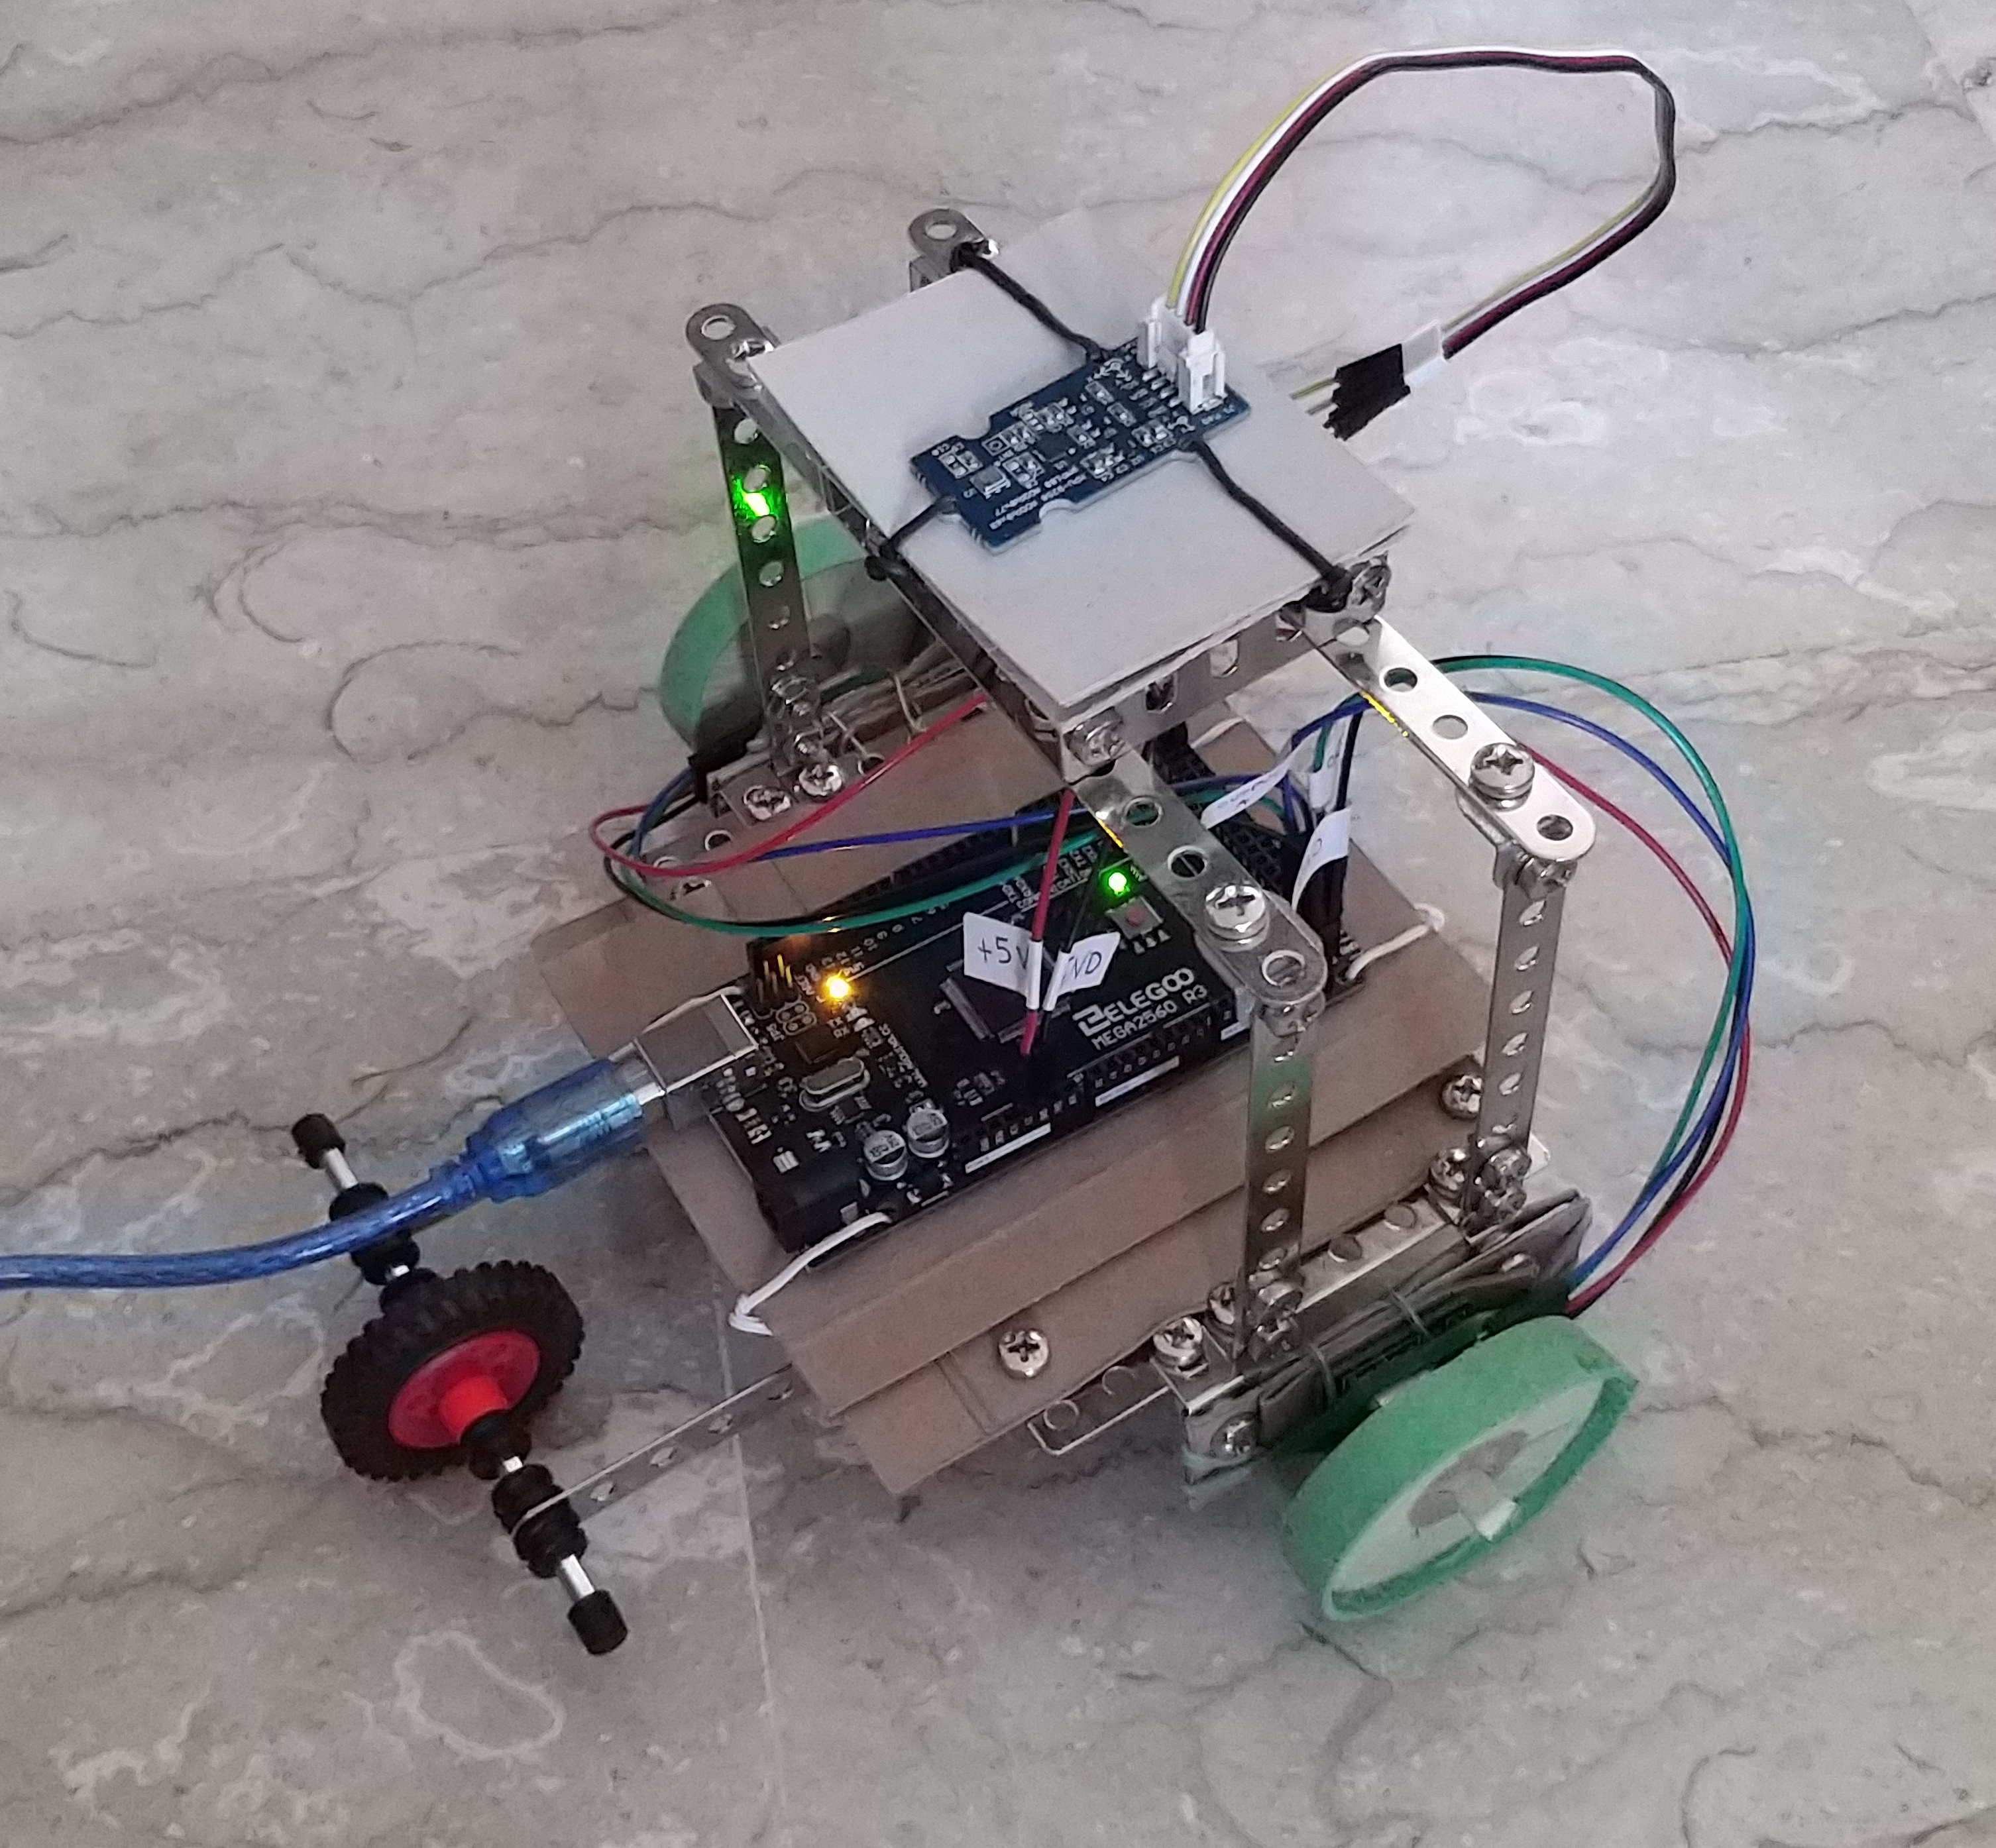
\includegraphics[width=\linewidth]{robot_image_06_20190701_085834}
	\end{subfigure}
	\captionsetup{justification=centering, margin=1.5cm}
	\centering
	\caption{Robot used for the tests.}
\end{figure}

\section{Communication Protocols}

In the development of the firmware we have used two communication protocols:
\begin{itemize}
	\item the I2C protocol to communicate with the IMU,
	\item the UART communication to interface with the host.
\end{itemize}
\subsection{I2C Protocol}

The I2C\footnote{I2C stands for Inter-Integrated Circuit} protocol is a synchronous serial computer bus. It enables multi-slave and multi-master modes, but we have used it in a simple configuration using the MEGA2560 board as master and the IMU as slave.\\

Each device on the bus has a preset ID so that the master can choose the slave to communicate with.\\
This bus uses two wires:
\begin{itemize}
	\item Serial Clock (SCL) for the clock signal (generated by the master) which synchronizes the communication between master and slave,
	\item Serial Data (SDA) carrying the data.
\end{itemize}

\begin{figure}[!ht]
	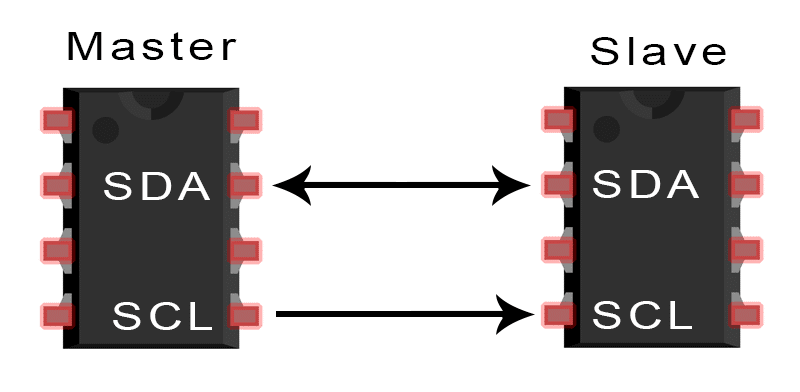
\includegraphics[scale=0.6]{i2c_master_slave}
	\captionsetup{justification=centering, margin=1.5cm}
	\centering
	\caption{I2C wires.}
	\centering
\end{figure}


The data signal is transferred in sequences of 8 bits, each of them synchronized with the clock signal.
\begin{itemize}
	\item The communication starts with the master sending a special START condition over the bus,
	\item then the master sends an 8-bit sequence indicating the address of the slave device to which the communication is addressed,
	\item at this point the master waits for the slave to send back an Acknowledgement (ACK).
	\item After this first Acknowledgement by the slave device, in most cases there is a second addressing sequence indicating the address of the internal register where to read or write.
	\item Finally the data is sent through the bus,
	\item and the communication ends with a STOP condition generated by the master.
\end{itemize}
\begin{figure}[!ht]
	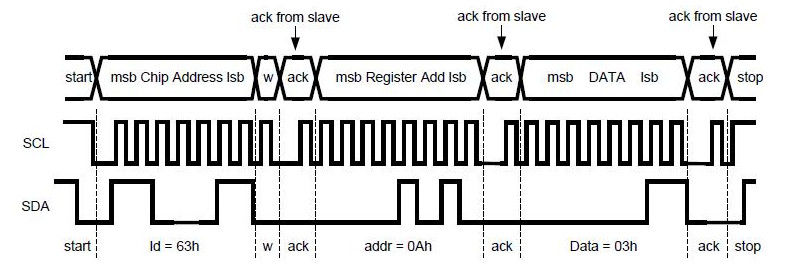
\includegraphics[scale=0.5]{i2c_protocol_01}
	\captionsetup{justification=centering, margin=1.5cm}
	\centering
	\caption{I2C general protocol.}
	\centering
\end{figure}

Let us now dig further in the protocol distinguishing the cases of reading and writing a register. To distinguish between a read and a write operation, in the first addressing cycle only the first 7 bits are actually used to identify the slave device, while the least significant bit is used to discriminate read and write operations [0 for a write operation, 1 for a read].
\begin{figure}[!ht]
	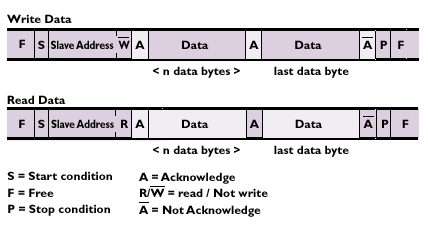
\includegraphics[scale=0.6]{i2c_protocol_02}
	\captionsetup{justification=centering, margin=1.5cm}
	\centering
	\caption{I2C protocol: distinguishing read and write operations.}
	\centering
\end{figure}

\paragraph{Write Operations}
A write operation is composed by a single write transaction, where the master sends two data bytes to the slave, the first one is the address of the internal register the master wants to write to, while the second one is the value the master wants to write in it.
\begin{itemize}
	\item[1. ] The master starts the transmission transmitting the start condition.
	\item[2. ] Then the master transmits the 7-bits device address, followed by the write bit (0), and waits for the slave to send an ACK.
	\item[3. ] At this point the master puts the address of the internal device register on the bus, and waits for the slave's ACK;
	\item[4. ] and next the master sends the data to be written, and waits for the slave's ACK. Eventually the master could go on sending more data which will be written in the following registers, waiting for the slave's ACK for each 8-bit data.
	\item[5. ] Finally the master transmits the stop condition to end the communication.
\end{itemize}

\paragraph{Read Operations}
A read operation is composed of a write transaction followed by a read transaction. In the write transaction the master sends to the slave the address of the register he wants to read, while in the read transaction the slave sends the value of the requested register to the master.
\begin{itemize}
	\item[1. ] The master starts the write transaction transmitting the start condition.
	\item[2. ] Then the master transmits the 7-bits device address, followed by the write bit (0), and waits for the slave to send an ACK;
	\item[3. ] and next the master puts the address of the internal device register on the bus, and waits for the slave's ACK.
	\item[4. ] At this point the master starts the read transaction retransmitting a start condition (restart).
	\item[5. ] Then the master transmits the 7-bits device address, followed by the read bit (1), and waits for the slave to send an ACK;
	\item[6. ] and next the slave puts the data to be read on the bus. The master will send an ACK only if more data (from the following registers) is expected, when the master does not want the slave to send more data on the bus it sends a NACK (Not-Acknowledgement). Therefore the slave will stop sending data only upon receiving a NACK.
	\item[7. ] Finally the master transmits the stop condition to end the communication.
\end{itemize}
See Appendix \ref{i2c_implementation} for an implementation of the I2C protocol.\\


\subsection{UART Communication}

The UART\footnote{UART stands for Universal Asynchronous Receiver-Transmitter} is a computer hardware device for asynchronous serial communication. It is not a communication protocol as I2C but a physical circuit on the microcontroller, whose main purpose is to transmit and receive serial data.\\

In UART communication, two devices communicate directly with each other. The transmitting UART converts parallel data into serial data, and then transmits it in serial to the receving UART, that is in charge of reconstructing the parallel data. Only two wires are used to transmit data between devices, each of them going from the Transmit (Tx) pin of a device to the Receive (Rx) pin of the other.

\begin{figure}[htb]
 \centering
	\begin{subfigure}{0.35\textwidth}
		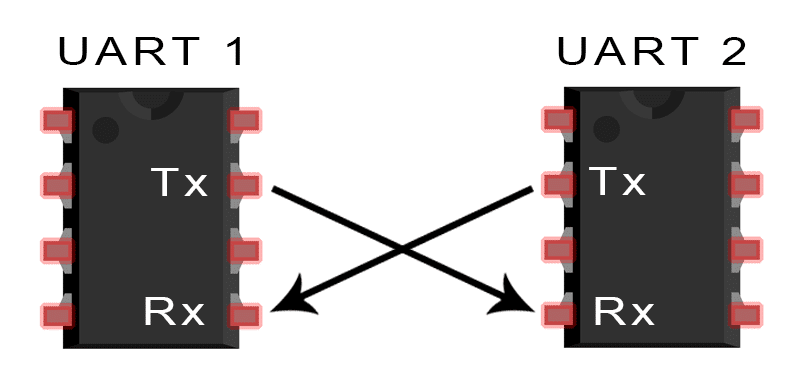
\includegraphics[width=\linewidth]{uart_tx_rx}
		\captionsetup{justification=centering}
		\caption{wires used for UART communication}
	\end{subfigure}\hfil
	\begin{subfigure}{0.6\textwidth}
		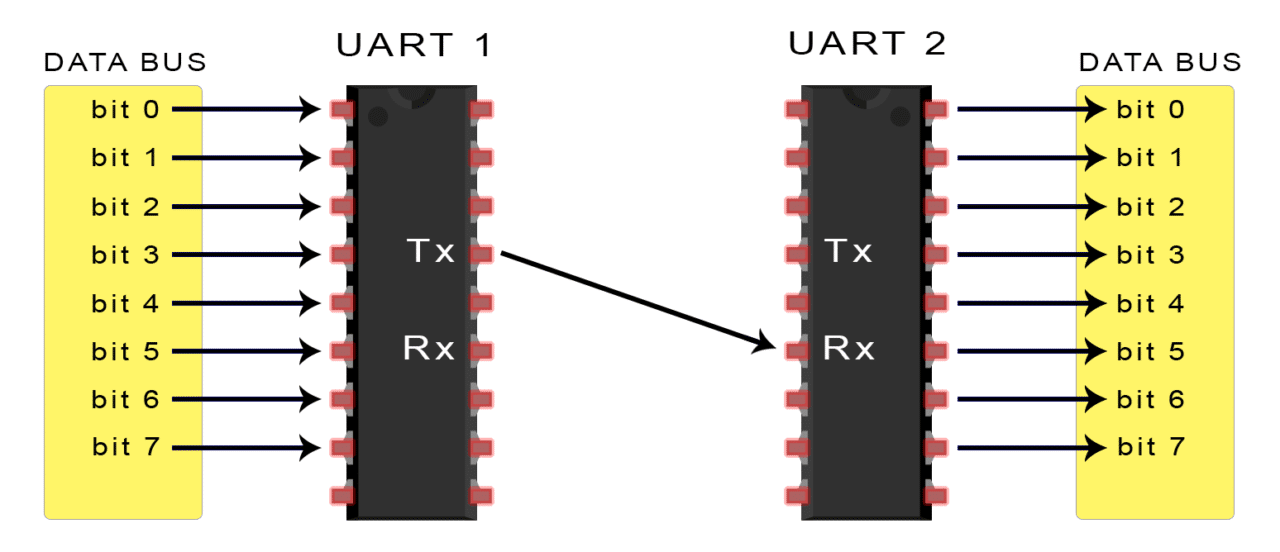
\includegraphics[width=\linewidth]{uart_parallel_to_serial}
		\captionsetup{justification=centering}
		\caption{parallel to serial data conversion for UART communication}
	\end{subfigure}
	\captionsetup{justification=centering, margin=1.5cm}
	\centering
	\caption{UART communication}
\end{figure}

\begin{itemize}
	\item[1. ] The transmitting CPU sends the data to be sent to the UART on a data bus, then the data is transferred from the data bus to the transmitting UART in parallel form.
	\item[2. ] The transmitting UART gets the parallel data from the bus and creates a data packet (adding a start bit, a parity bit and a stop bit).
					\begin{figure}[!ht]
						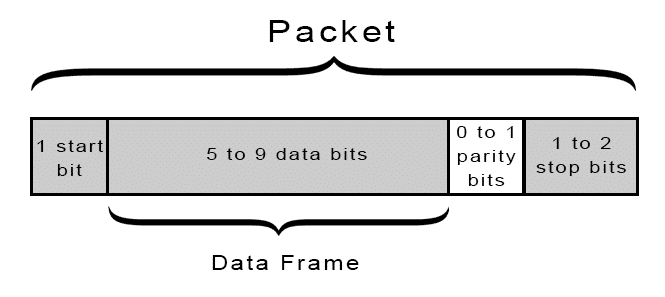
\includegraphics[scale=0.5]{uart_packet}
						\captionsetup{justification=centering, margin=1.5cm}
						\centering
						\caption{UART data packet.}
						\centering
					\end{figure}
	\item[3. ] The transmitting UART sends the data packet to the receiving UART serially, outputting it bit by bit from the Tx pin.
	\item[4. ] The receiving UART reads the packet bit by bit from the Rx pin,
	\item[5. ] and then converts the data received back into parallel form and removes the start bit, the parity bit and the stop bit.
	\item[6. ] Finally the receiving UART transfers the data to the receiving CPU on the data bus in parallel.
\end{itemize}
See Appendix \ref{uart_implementation} for an implementation of UART communication.\\

\section{Firmware}

All the firmware is designed to be interrupt driven. In addition to the interrupt driven implementation of the I2C protocol and the UART communication, the firmware's logic is based on timed interrupts. The sampling of the sensors and the update of the odometry is at a rate of 100 Hz, while the communication with the host is done at a rate of 1 Hz.

\subsection{Interpreting the Encoders Observations}

An encoder has two outputs A and B, which we have connected to two pins on the board.\\
When an encoder detects a rotation its outputs become two square waves (as described in \ref{encoders_how_they_work}), while when there is no rotation its outputs do not change their value. Therefore we have decided to use an interrupt solution, throwing an interrupt when one of the two pins changed its value.\\
We have connected the encoder corresponding to the left wheel to the pins 52-53 (PB1 and PB0 respectively\supercite{mega2560_datasheet}) while the one on the right wheel to the pins 50-51 (PB3 and PB2 respectively). Therefore we are using the first 4 pins of port B.
\begin{ccode}
	#define ENC_MASK 0xf //0b1111
	
	cli();

		//set the encoder pins as input
	DDRB &= ~ENC_MASK;
		//enable pull up resistors
	PORTB |= ENC_MASK;
		//set interrupt on change, looking up PCMSK0
	PCICR |= (1 << PCIE0);
		//tells which bits of the port triggers the interrupt
	PCMSK0 |= ENC_MASK;

	sei();
\end{ccode}
\captionof{lstlisting}{Installing the interrupt for handling the encoders.}

The ISR will then be responsible for the update of the state of the encoders. For each encoder we need to store:
\begin{itemize}
	\item a global counter, counting the total number of rotations the encoder has been subject to. Note that clockwise rotations increment the counter, while anticlockwise rotations decrement it.
	\item the previous value of the output pins, since in an incremental encoder the sense of the rotation is encoded in the transition between states.
\end{itemize}
\begin{ccode}
	typedef struct Encoder_t {
		uint8_t prev_value;	// previous value of the output pins
		int32_t counter;		// global counter of the encoder
	} Encoder_t;
\end{ccode}
\captionof{lstlisting}{Structure used to store all useful informations about encoders.}

Therefore the ISR recovers the actual and the previous values of the output pins and uses them to lookup in a transition table and update the encoder rotation counter.
\begin{ccode}
	#define NUM_ENCODERS 2
	
		//global variable storing the current state of the encoders
			//updated by the ISR
	static Encoder_t Encs[NUM_ENCODERS];
	
	static const int8_t _transition_table []= {
			0,	//0000
		 -1,	//0001
			1,	//0010
			0,	//0011
			1,	//0100
			0,	//0101
			0,	//0110
		 -1,	//0111
		 -1,	//1000
			0,	//1001
			0,	//1010
			1,	//1011
			0,	//1100
			1,	//1101
		 -1,	//1110
			0		//1111
	};

	// Interrupt Service Routine for PCINT0
	ISR(PCINT0_vect) {
		uint8_t port_value = PINB & ENC_MASK;
	
		uint8_t i;
		for(i=0; i<NUM_ENCODERS; i++){
				//we need the previous state, since in incremental encoders
					//we handle transitions from a state to the next
			Encs[i].prev_value <<=2;
			
				// port_value stores the new values of all encoders
					// with &0x03 we can handle an encoder at the time
					// and with >>= 2 t the end, we pass to the next encoder
			Encs[i].prev_value = Encs[i].prev_value | (port_value & 0x03);
			Encs[i].counter += _transition_table[Encs[i].prev_value & 0x0F];
		
			port_value >>= 2;
		}
	}
\end{ccode}
\captionof{lstlisting}{Installing the interrupt for handling the encoders.}


\subsection{Interpreting the IMU Observations}\label{imu_calib}

The IMU MPU9250 provides an I2C interface, through which we can access its control register and its 16-bit digital output registers\supercite{imu_prod_spec}.\\

\subsubsection{Initializing the IMU}

Reading the IMU datasheet\supercite{imu_prod_spec} and the register map\supercite{imu_regs} we were able to initialize the configuration registers according to our needs.\\

The gyroscope's full scale range was set to 250 DPS\footnote{DPS stands for Degrees Per Second}, hence it can observe only angular velocities in the range [-250 DPS, +250 DPS]. The accelerometer's full scale range instead was set to 2 G\footnote{1 G corresponds to the gravitational acceleration (i.e. $\sim 9.8 m/s^2$)} and therefore it can measure accelerations in the range [-2 G, +2 G].\\These are a quite small ranges but perfect for our needs since we do not expect the robot to exceed these bounds; moreover the use of small ranges gives us high sensitivity in these ranges.\\

The gyroscope's bandwidth, which is the highest frequency of angular velocity variation that can be detected by the sensor, was set to 41 Hz. The accelerometer's bandwidth instead was set to 44.8 Hz.\\According to the Nyquist Sampling Criterion, the rate at which the sensors are sampled must be at least twice the sensors' bandwidths. Therefore since we want to sample the IMU sensors at 100 Hz, we had to set the sensors' bandwidths below 50 Hz.
\begin{ccode}
	static void IMU_ConfigRegs(void) {
		//resets the internal registers and restores the default settings
		I2C_WriteRegister(ACCELGYRO_DEVICE, PWR_MGMT_1, 0x80);
		_delay_ms(500);
		
		//sets Gyroscope Full Scale range to 250dps (degrees/sec)
			//[low range, high sensitivity]
		I2C_WriteRegister(ACCELGYRO_DEVICE, GYRO_CONFIG, 0x00);
		_delay_ms(10);
	
		//sets Gyroscope bandwidth to 41Hz,
		I2C_WriteRegister(ACCELGYRO_DEVICE, CONFIG, 0x03);//41 Hz
		_delay_ms(10);
	
		//sets Accelerometer Full Scale to 2G
		I2C_WriteRegister(ACCELGYRO_DEVICE, ACCEL_CONFIG, 0x00);
		_delay_ms(10);
		
		//sets Accelerometer bandwidth to 44.8 Hz
		I2C_WriteRegister(ACCELGYRO_DEVICE, ACCEL_CONFIG2, 0x03);//44.8 Hz
		_delay_ms(10);

		//sets PowerManagement Registers
			//auto selects the best available clock source
			//and disables the sleep mode
		I2C_WriteRegister(ACCELGYRO_DEVICE, PWR_MGMT_1, 0x01);
		_delay_ms(10);
		
		//sets all sensors to on
		I2C_WriteRegister(ACCELGYRO_DEVICE, PWR_MGMT_2, 0x00);
		_delay_ms(10);
	
		//i2c_master interface pins(SCL, SDA)
			//will go into "bypass mode"
			//when the i2c master interface is disabled
		I2C_WriteRegister(ACCELGYRO_DEVICE, INT_PIN_CFG, 0x02);
		_delay_ms(10);
	}
\end{ccode}
\captionof{lstlisting}{IMU initialization of configuration registers.}

\subsubsection{Reading IMU registers}

As mentioned in the previous paragraph, we want to sample the IMU sensors at a rate of 100 Hz. Therefore we defined a timed interrupt with a frequency of 100 Hz and we gave to the corresponding interrupt service routine the task of reading the IMU data registers.
\begin{ccode}
	#define IMU_UPDATE_RATE 100 //Hz

	//from a frequency in Hz, we get a period in millisecs
 uint16_t period_ms = 1000 / IMU_UPDATE_RATE;
 
 //configure timer3, prescaler : 256, CTC (Clear Timer on Compare match)
 TCCR3A = 0;
 TCCR3B = (1 << WGM12) | (1 << CS12); 
 
 /*
	 * cpu frequency 16MHz = 16.000.000 Hz
	 * prescaler 256
	 *	-->> TCNT3 is increased at a frequency of 16.000.000/256 Hz = 62500 Hz
	 *	so 1 ms will correspond do 62.5 counts
	 */
 OCR3A = (uint16_t)(62.5 * period_ms);

	// timer-interrupt enabling must be executed atomically (no other interrupts)
		// and ATOMIC_FORCEON ensures Global Interrupt Status flag bit in SREG set afetrwards
 ATOMIC_BLOCK(ATOMIC_FORCEON) {
 	TIMSK3 |= (1 << OCIE3A);
 }
\end{ccode}
\captionof{lstlisting}{Installing the timed-interrupt to periodically read the IMU data registers.}

\begin{ccode}
	ISR(TIMER3_COMPA_vect) {
		//reads the accelerometer and the gyroscope data registers
		IMU_AccelGyroRaw();

		//increases the time stamp
		IMU.imu_time_seq++;
	}
\end{ccode}
\captionof{lstlisting}{ISR in charge of reading the IMU data registers.}

The output data from the accelerometer and the gyroscope are 16-bit values for each axis, divided in two 8-bit registers. Since the 6 registers for the accelerometer and the six ones for the gyroscope are consecutive, we can read them in a single I2C communication cycle and then reconstruct the 16-bit digital values.

\subsubsection{Calibrating the IMU sensors}

As described in paragraph \ref{mems_errors}, MEMS sensors are subject to errors, some of which can be compensated through a prior calibration process\supercite{imu_calib_01}\supercite{imu_calib_02}.\\

To compensate constant bias errors for the accelerometer and the gyroscope, we calculate the calibration biases by taking a long term average of the sensors' outputs while the IMU is motionless.\\
To compensate the scale factor errors of the accelerometer, we use a very simple multi-position scheme. By keeping the IMU with its z-axis upwards (aligned with the vertical gravity field) we expect to measure an acceleration of 1 G along the z-axis; therefore we can use the digital output of the sensor as the scale factor of the z-axis. By aligning the other axes with the gravity field, we calculate the scale factors for all the other axes of the accelerometer.\\
We have calculated the scale factors of the gyroscope starting from the full scale range. Since we expect the full scale range to correspond to the maximum value of the digital output, we have calculated the scale factor by dividing the maximum digital value by the maximum physically meaningful value than can be measured: $scale\_factor = 2^{15} / 250$. We did not compensate the scale factor errors of the gyroscope.\\

\begin{ccode}
	#define CALIBRATION_SAMPLES	128
	#define CALIBRATION_SAMPLES_LOG	7

	#define IMU_POS_Z_UP 0 // z-axis upwards
	#define IMU_POS_X_UP 1 // x-axis upwards
	#define IMU_POS_Y_UP 2 // y-axis upwards
	#define IMU_POS_Z_DOWN 3 // z-axis downwards
	#define IMU_POS_X_DOWN 4 // x-axis downwards
	#define IMU_POS_Y_DOWN 5 // y-axis downwards
	#define IMU_N_POS 6 //max number if positions
	
	int32_t gyro_x_sum[IMU_N_POS]={}, gyro_y_sum[IMU_N_POS]={}, gyro_z_sum[IMU_N_POS]={};
	int32_t accel_x_sum[IMU_N_POS]={}, accel_y_sum[IMU_N_POS]={}, accel_z_sum[IMU_N_POS]={};
	
	uint8_t p, i, orientation;
	
	for(p=0; p < IMU_N_POS; p++) {
		//waits for the robot is in a new orientation
			// ...
		
		//sets ths local variable to the current IMU orientation
		orientation = <imu_orientation>;
			
		//get samples
		for(i=0; i<CALIBRATION_SAMPLES; i++) {	
			gyro_x_sum[orientation] += <gyro_raw_x_observation>;
			gyro_y_sum[orientation] += <gyro_raw_y_observation>;
			gyro_z_sum[orientation] += <gyro_raw_z_observation>;
			
			accel_x_sum[orientation] += <accel_raw_x_observation>;
			accel_y_sum[orientation] += <accel_raw_y_observation>;
			accel_z_sum[orientation] += <accel_raw_z_observation>;
		}

		gyro_x_sum[orientation] >>= CALIBRATION_SAMPLES_LOG;
		gyro_y_sum[orientation] >>= CALIBRATION_SAMPLES_LOG;
		gyro_z_sum[orientation] >>= CALIBRATION_SAMPLES_LOG;

		accel_x_sum[orientation] >>= CALIBRATION_SAMPLES_LOG;
		accel_y_sum[orientation] >>= CALIBRATION_SAMPLES_LOG;
		accel_z_sum[orientation] >>= CALIBRATION_SAMPLES_LOG;
	}
	
	// GYROSCOPE
	int32_t gyro_total_x_sum=0, gyro_total_y_sum=0, gyro_total_z_sum=0;
	for(p=0; p<6; p++) {
		gyro_total_x_sum += gyro_x_sum[p];
		gyro_total_y_sum += gyro_y_sum[p];
		gyro_total_z_sum += gyro_z_sum[p];
	}
	
		//calculates the gyro's constant biases
	int32_t gyro_x_bias = (int16_t)(gyro_total_x_sum / 6);
	int32_t gyro_y_bias = (int16_t)(gyro_total_y_sum / 6);
	int32_t gyro_z_bias = (int16_t)(gyro_total_z_sum / 6);
	
		//calculates the gyro's scale factor (no calibration)
	float gyro_sensitivity = (float)((uint16_t)(1<<15) / 250.);

	float gyro_x_scale = gyro_sensitivity;
	float gyro_y_scale = gyro_sensitivity;
	float gyro_z_scale = gyro_sensitivity;
	
	//ACCELEROMETER	
	//asse X
		//to calculate the bias, we take in consideration the positions where we expect zero-acceleration along the axis
	int32_t accel_x_bias_sum = accel_x_sum[IMU_POS_Z_UP]+accel_x_sum[IMU_POS_Y_UP]+accel_x_sum[IMU_POS_Z_DOWN]+accel_x_sum[IMU_POS_Y_DOWN];
		//to calculate the scale factor, we take in consideration the positions with +1G and -1G acceleration
	int32_t accel_x_scale_sum = accel_x_sum[IMU_POS_X_UP]-accel_x_sum[IMU_POS_X_DOWN];
	
	//asse Y
	int32_t accel_y_bias_sum = accel_y_sum[IMU_POS_Z_UP]+accel_y_sum[IMU_POS_X_UP]+accel_y_sum[IMU_POS_Z_DOWN]+accel_y_sum[IMU_POS_X_DOWN];
	int32_t accel_y_scale_sum = accel_y_sum[IMU_POS_Y_UP]-accel_y_sum[IMU_POS_Y_DOWN];
	
	//asse Z
	int32_t accel_z_bias_sum = accel_z_sum[IMU_POS_X_UP]+accel_z_sum[IMU_POS_Y_UP]+accel_z_sum[IMU_POS_X_DOWN]+accel_z_sum[IMU_POS_Y_DOWN];
	int32_t accel_z_scale_sum = accel_z_sum[IMU_POS_Z_UP]-accel_z_sum[IMU_POS_Z_DOWN];
	
		//calculates the accel's constant biases
	int32_t accel_x_bias = (int16_t)(accel_x_bias_sum >> 2);
	int32_t accel_y_bias = (int16_t)(accel_y_bias_sum >> 2);
	int32_t accel_z_bias = (int16_t)(accel_z_bias_sum >> 2);
	
		//calculates the accel's scale factor
			// we must not keep track of bias calculating the scale
				//because we are subtracting two accel_x_sum values ( one positive, one negative )
					//accel_x_scale_sum = accel_x_sum[IMU_POS_X_UP] - accel_x_sum[IMU_POS_X_DOWN];
						//we would have +BIAS the first time, and -BIAS the second
					//and the two biases goes away
	float accel_x_scale = (float)(accel_x_scale_sum >> 1);
	float accel_y_scale = (float)(accel_y_scale_sum >> 1);
	float accel_z_scale = (float)(accel_z_scale_sum >> 1);
\end{ccode}
\captionof{lstlisting}{Accelerometer and Gyroscope Calibration.}

\subsubsection{Interpreting values read from the registers}

Upon receipt of a 16-bit digital value, we must convert it to a physically meaningful value.\\
First of all we subtract the calibration bias, then we divide the 16-bit digital value for the scale factor calculated during the calibration.
\begin{ccode}
	//in accel_raw_x, accel_raw_y, accel_raw_z we store the 16-bit values read from the sensor
	//while in accel_x, accel_y, accel_z we store physically meaningful values

	accel_x = (float)(accel_raw_x - accel_x_bias) / accel_x_scale_factor;
	accel_y = (float)(accel_raw_y - accel_y_bias) / accel_y_scale_factor;
	accel_z = (float)(accel_raw_z - accel_z_bias) / accel_z_scale_factor;
\end{ccode}
\captionof{lstlisting}{Converting the 16-bit digital accelerometer values to physically meaningful values (i.e. accelerations). [Similarly it can be done for the gyroscope.]}


\subsection{Communication with the Host}

The communication with the host is packet-based and performed via UART communication. At a frequency of 1 Hz the firmware sends to the host the estimated position using differential drive and the one estimated using inertial navigation.\\
\begin{ccode}
	typedef uint8_t PacketType;
	typedef uint8_t PacketSize;
	typedef uint16_t PacketSeq;   

	#pragma pack(push, 1)
	typedef struct {
		PacketType type; // type of the packet
		PacketSize size; // size of the packet in bytes
		PacketSeq seq;		// sequential number
	} PacketHeader;

	typedef struct {
		PacketHeader header;
		
		//packet-specific data
		//...
	} ExamplePacket;
	#pragma pack(pop)
\end{ccode}
\captionof{lstlisting}{Structure of the packets used for Firmware-Host Communication via UART.}

\section{Host}

The host has a multi-thread structure. There is a comunication thread in charge of listening to the serial port and storing the information sent by the firmware and the main thread which is just logging the data received on the screen at a rate of 1 Hz.\\

\subsection{Serial Interface}

On the host the serial is accessible at \textit{/dev/ttyACM0}. We have used the \textit{termios} interface to configure it.\\
\begin{ccode}
	#define SERIAL_NAME "/dev/ttyACM0"
	
	int fd = open(SERIAL_NAME, O_RDWR | O_NOCTTY | O_SYNC);
\end{ccode}
\captionof{lstlisting}{Opening the Serial as a file.}

\begin{ccode}
	#define SERIAL_SPEED 57600
	#define SERIAL_PARITY 0
	
	struct termios tty;
	memset(&tty, 0, sizeof(tty));
	
	// store in tty the parameters associated to the serial device referred by fd
	res = tcgetattr(fd, &tty);
	//... check res >= 0
	
	//converts speed into one of the speed_t Bnnn constants
	speed_t speed_bnnn = B0;
	switch (speed){
		case 19200:
			speed_bnnn=B19200;
			break;
		case 38400:
			speed_bnnn=B38400;
			break;
		case 57600:
			speed_bnnn=B57600;
			break;
		case 115200:
			speed_bnnn=B115200;
			break;
		default:
			printf("[serial_set_interface_attribs] Cannot set baudrate to %d\n", speed);
			return -1;
	}	
	// sets the input baud rate stored in the termios structure to speed
	cfsetispeed(&tty, speed_bnnn);
	// sets the output baud rate stored in the termios structure to speed
	cfsetospeed(&tty, speed_bnnn);
	
	// sets the terminal to a "raw" mode
		// input is available character by character, echoing is disabled
		// all special processing of terminal input and output characters is disabled. 
		// serial switchs to noncanonical mode
	cfmakeraw(&tty);
	
	// PARENB : Enable parity generation on output and parity checking for input.
	// PARODD : If set, then parity for input and output is odd;
									//otherwise even parity is used.
	if( parity )
		tty.c_cflag |= (PARENB | PARODD);
	else
		tty.c_cflag &= ~PARENB;
	
	// sets characters' size to 8-bit
	tty.c_cflag &= ~CSIZE;
	tty.c_cflag |= CS8;
	
	// set blocking mode
		// MIN > 0; TIME > 0:
			// TIME specifies the limit for a timer in tenths of a second.
				// Once an initial byte of input becomes available,
					//timer is restarted after each further byte is received.
			// read returns either
				// when min {number of bytes requested, MIN bytes have been read }
				// when the inter-byte timeout expires.
			// Because the timer is only started after the initial byte
				// becomes available, at least one byte will be read.
	tty.c_cc[VMIN] = 1;
	tty.c_cc[VTIME] = 5; // 0.5 seconds read timeout
	
	// sets the parameters associated with the serial device
		// from the termios structure tty
		// TCSANOW : the change occurs immediately
	res = tcsetattr(fd, TCSANOW, &tty);
	//... check res >= 0
\end{ccode}
\captionof{lstlisting}{Configuration of the serial interface.}

Using this configuration it is possible to perform read and write operations on the serial as if it was a local file on the host.

\subsection{ROS node}

Furthermore we also provide a ROS node interfacing with the ROS environment. This node publishes the two odometries on two different topics so that they can be easily visualized in RViz\footnote{RViz is the ROS visualization tool}.
\begin{figure}[!ht]
	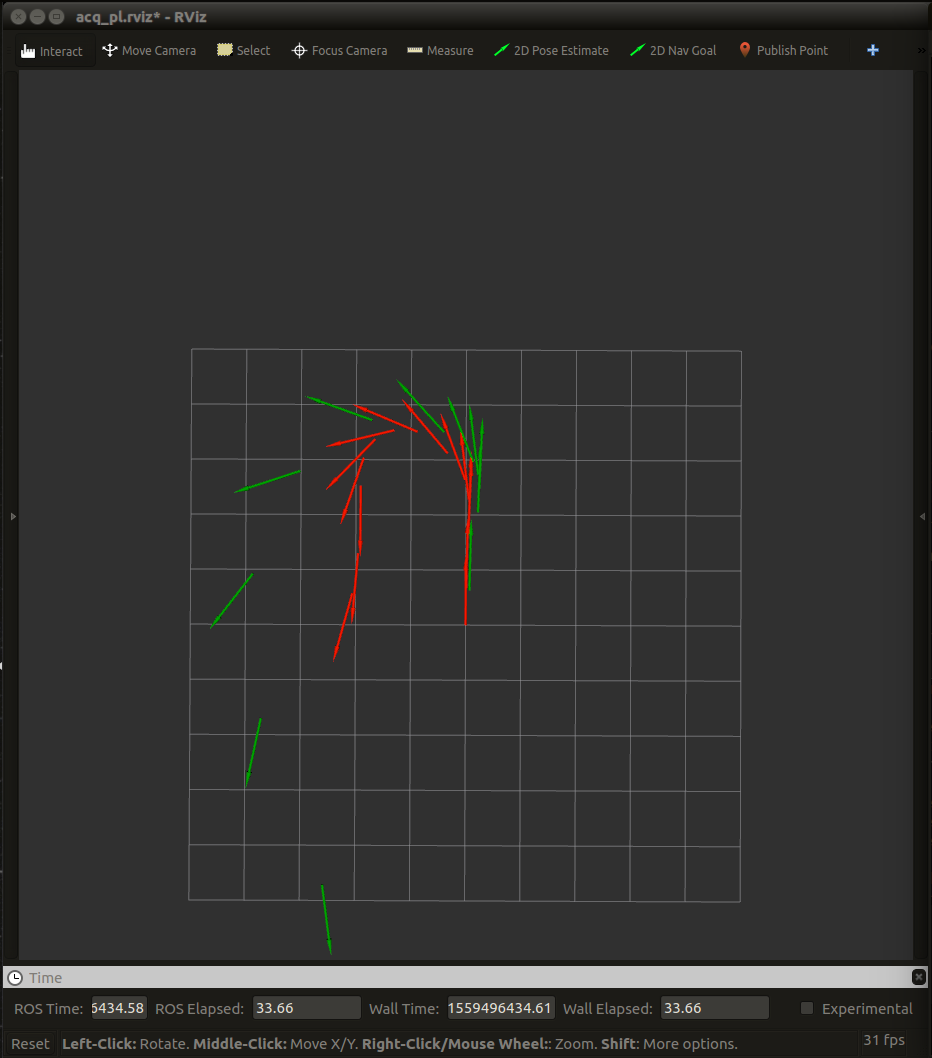
\includegraphics[scale=0.25]{rviz_sample}
	\captionsetup{justification=centering, margin=1.5cm}
	\centering
	\caption{Data Visualization in RViz. In red we are plotting the position estimated using differential drive, while in green the one using inertial navigation.}
	\centering
\end{figure}
